\documentclass[a4paper, 12pt]{article}
\usepackage{eurosym}
\usepackage{pdflscape}
\usepackage{pgfgantt}
\usepackage{pgfplots}


\newcommand{\templates}{../../template}
\usepackage[a4paper, margin=2.5cm]{geometry}

\usepackage{enumitem}
\setlist[itemize]{noitemsep}
\setlist[enumerate]{noitemsep}

\let\oldpar\paragraph
\renewcommand{\paragraph}[1]{\oldpar{#1\\}\noindent}

% Avoid dots in the table of contents, it mess with the gulpease calculation
\makeatletter
\renewcommand{\@dotsep}{10000} 
\makeatother
\usepackage{graphicx}
\usepackage{hyperref}
\usepackage{makecell}
\usepackage{fancyhdr}

\newcommand{\settitolo}[1]{\newcommand{\titolo}{#1\\}}
\newcommand{\setprogetto}[1]{\newcommand{\progetto}{#1\\}}
\newcommand{\setcommittenti}[1]{\newcommand{\committenti}{#1\\}}
\newcommand{\setredattori}[1]{\newcommand{\redattori}{#1\\}}
\newcommand{\setrevisori}[1]{\newcommand{\revisori}{#1\\}}
\newcommand{\setresponsabili}[1]{\newcommand{\responsabili}{#1\\}}
\newcommand{\setversione}[1]{
	\ifdefined\versione\renewcommand{\versione}{#1\\}
	\else\newcommand{\versione}{#1\\}\fi
}
\newcommand{\setdestuso}[1]{\newcommand{\uso}{#1\\}}
\newcommand{\setdescrizione}[1]{\newcommand{\descrizione}{#1\\}}

\newcommand{\makefrontpage}{
	\begin{titlepage}
		\begin{center}

		
\includegraphics[width=0.4\textwidth]{\templates/4ourSquared_logo}\\

		{\Large 4OURSQUARED}\\[6pt]
		\href{mailto://4oursquared.unipd@gmail.com}{4oursquared.unipd@gmail.com}\\
		
		\ifdefined\progetto
		\vspace{1cm}
		{\Large\progetto}
		{\large\committenti}
		\else\fi
		
		\vspace{1.5cm}
		{\LARGE\titolo}
		
		\vfill
		
		\begin{tabular}{r | l}
		\multicolumn{2}{c}{\textit{Informazioni}}\\
		\hline
		
		\ifdefined\redattori
			\textit{Redattori} &
			\makecell[l]{\redattori}\\
		\else\fi
		\ifdefined\revisori
			\textit{Revisori} &
			\makecell[l]{\revisori}\\
		\else\fi
		\ifdefined\responsabili
			\textit{Responsabili} &
			\makecell[l]{\responsabili}\\
		\else\fi
		
		\ifdefined\versione
			\textit{Versione} & \versione
		\else\fi
		
		\textit{Uso} & \uso
		
		\end{tabular}
		
		\vspace{2cm}
		
		\ifdefined\descrizione
		Descrizione
		\vspace{6pt}
		\hrule
		\descrizione
		\else\fi
		\end{center}
	\end{titlepage}
}
\usepackage{hyperref}
\usepackage{array}
\usepackage{tabularx}
\usepackage{adjustbox}

\newcounter{verscount}
\setcounter{verscount}{0}
\newcommand{\addversione}[5]{
	\ifdefined\setversione
		\setversione{#1}
	\else\fi
	\stepcounter{verscount}
	\expandafter\newcommand%
		\csname ver\theverscount \endcsname{#1&#2&#3&#4&#5}
}

\newcommand{\listversioni}{
	\ifnum\value{verscount}>1
		\csname ver\theverscount \endcsname
		\addtocounter{verscount}{-1}
		\\\hline
		\listversioni
	\else
		\csname ver\theverscount \endcsname\\\hline
	\fi
}

\newcommand{\makeversioni}{
	\begin{center}
		\begin{tabularx}{\textwidth}{|c|c|c|c|X|}
		\hline
		\textbf{Versione} & \textbf{Data} & \textbf{Redattore} & \textbf{Verificatore} & \textbf{Descrizione} \\
		\hline
		\listversioni
		\end{tabularx}
	\end{center}
	\clearpage
}
\graphicspath{ {./immagini/} }

\settitolo{Piano di Progetto}
\setredattori{Alberti Nicolas \\ Brotto Romina \\ Cavaliere Erica \\ Soldà Matteo}
\setdestuso{esterno}
\setdescrizione{
Questo documento serve a tracciare l'efficienza del progetto. Tiene traccia dei costi sostenuti fino ad oggi e li confronta con i costi preventivati, in relazione agli obiettivi fissati.
}

\addversione{0.0.1}{22/04/2023}{Cavaliere Erica}{Alberti Nicolas}{Stesura iniziale}
\addversione{0.0.2}{24/04/2023}{Cavaliere Erica}{Soldà Matteo}{Correzione errori e aggiunta delle intestazioni e dei piè di pagina}
\addversione{0.0.3}{26/04/2023}{Cavaliere Erica}{Brotto Romina}{Inserimento interruzioni di pagina e completamento grafico di Gantt}
\addversione{0.0.4}{16/05/2023}{Cavaliere Erica}{Salami Lorenzo}{Inserimento degli sprint e aggiornamento dei grafici di Gantt}
\addversione{0.0.5}{25/05/2023}{Alberti Nicolas}{Cavaliere Erica}{Inserimento dello sprint 4; aggiornamento dei grafici di Gantt}
\addversione{0.0.6}{02/06/2023}{Brotto Romina}{Soldà Matteo}{Completamento sprint 5}
\addversione{0.0.7}{11/06/2023}{Cavaliere Erica}{Soldà Matteo}{Completamento sprint 6}
\addversione{0.0.8}{23/06/2023}{Alberti Nicolas}{Cavaliere Erica}{Completamento sprint 7}
\addversione{0.0.9}{02/07/2023}{Soldà Matteo}{Cavaliere Erica}{Completamento sprint 8}

\def\pgfcalendarmonthitname#1{%
\ifcase#1 \or Gennaio\or Febbraio\or Marzo\or Aprile\or Maggio\or Giugno\or Luglio\or Agosto\or Settembre\or Ottobre\or Novembre\or Dicembre\fi%
}
\usepgfplotslibrary{dateplot}

\begin{document}
\makeindexdetails
\makefrontpage \makeversioni
\tableofcontents
\newpage
\clearpage
\makecontentsdetails{Piano di Progetto} 

\section{Analisi dei rischi}

\subsection{Rischi tecnologici}
Le tecnologie consigliate per lo svolgimento del progetto da parte del richiedente possono risultare nuove per alcuni componenti del gruppo, questo può portare difficoltà nell'utilizzo delle tecnologie, portando di conseguenza errori nel codice e ritardi di consegna. \newline
Per prefissare le scadenze bisognerà tenere conto del tempo impiegato per imparare le nuove tecnologie, oltre al tempo di sviluppo del progetto stesso.

\subsection{Rischi organizzativi}
Durante lo svolgimento del progetto, è possibile andare incontro a dei problemi di organizzazione degli orari e quindi di non riuscire a rispettare la stima delle ore richiesta e, di conseguenza, sforare i costi indicati dal preventivo iniziale.
\newpage
\section{Pianificazione del lavoro}

\subsection{Lavoro svolto}
%Di seguito sono riportati i grafici aggiornati del lavoro pianificato.\newline
%Se si desidera vedere l'evoluzione degli impegni presi in un arco temporale preciso, lo si può vedere nella sezione \ref{Scrum}.\newline



\begin{itemize}
    \item Way of Working\newline
    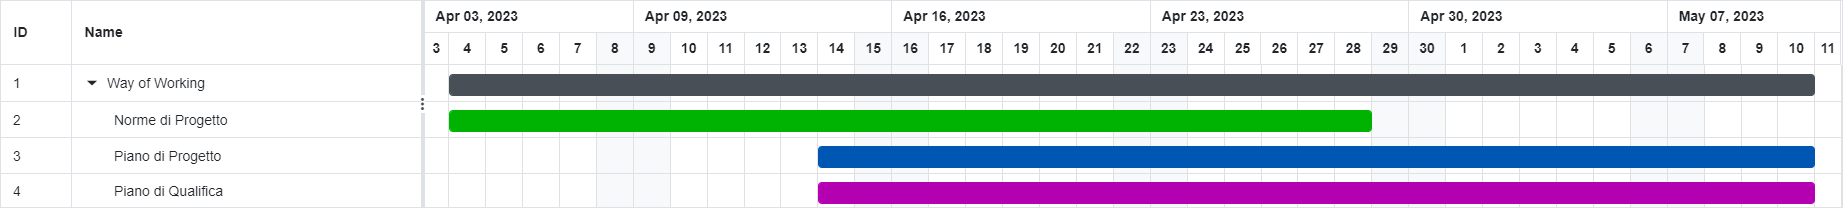
\includegraphics[scale=0.24]{WoW_2.png}\newline
    \item Requirements and Technology Baseline\newline
    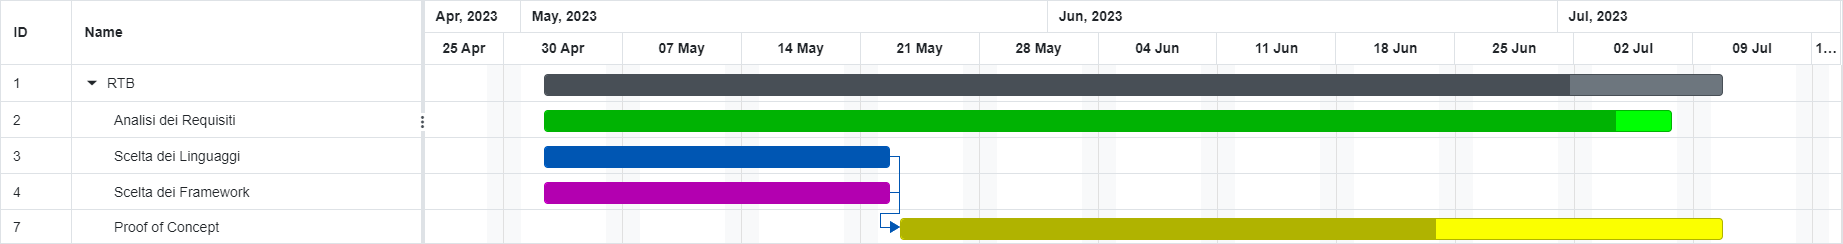
\includegraphics[scale=0.24]{RTB_7.png}\newline
\end{itemize}

\subsection{Scrum}\label{Scrum}

\subsubsection{Sprint 1}
\textbf{Data di inizio:} 14/04/2023\newline
\textbf{Data di fine:} 27/04/2023\newline
\newline
\textbf{Suddivisione del lavoro:}
\begin{itemize}
    \item aggiornamento delle norme di progetto;
    \item stesura del piano di progetto;
    \item stesura del piano di qualifica.
\end{itemize}
\textbf{Difficoltà incontrate:}
\begin{itemize}
    \item problemi a suddividere i ruoli e assegnare i compiti.
\end{itemize}
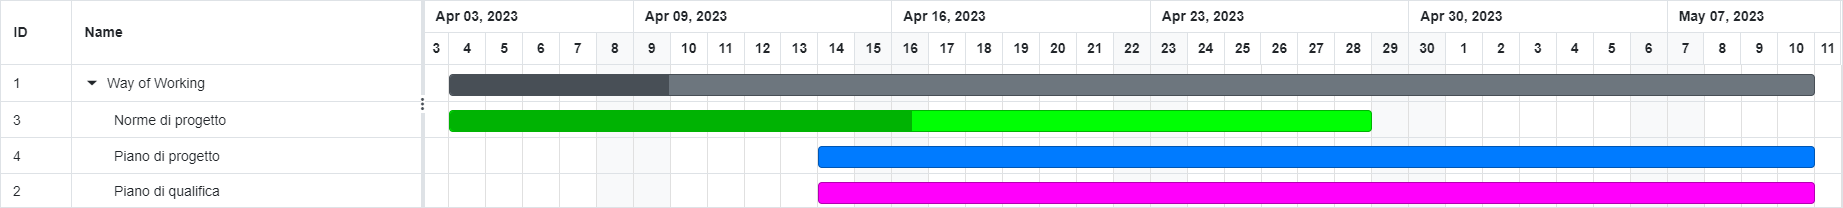
\includegraphics[scale=0.24]{WoW_1.png}\newline
\newline
\begin{tabular}{|c|c|c|c|c|c|c|c|}
    \hline
    \textbf{ORE} & \textbf{Respon.} & \textbf{Amministr.} & \textbf{Analista} & \textbf{Proget.} & \textbf{Program.} & \textbf{Verif.} & \textbf{Totale}\\
    \hline
    Erica & & & 1 & & & & 1\\
    \hline
    Francesco & & 1 & & & & & 1\\
    \hline
    Lorenzo & & & 1 & & & & 1\\
    \hline
    Matteo & 2 & & & & & & 2\\
    \hline
    Nicolas & & 1.30 & & & & & 1.30\\
    \hline
    Romina & & & & & & 1 & 1\\
    \hline
    \textbf{Totale} & 2 & 2.30 & 2 & 0 & 0 & 1 & 7.30\\
    \hline
\end{tabular}\\[8pt]

\subsubsection{Sprint 2}
\textbf{Data di inizio:} 28/04/2023\newline
\textbf{Data di fine:} 08/05/2023\newline
\newline
\textbf{Suddivisione del lavoro:}
\begin{itemize}
    \item aggiornamento delle Norme di Progetto inserendo la gestione dei processi e il ticketing;
    \item creare una prima stesura dell'Analisi dei Requisiti;
    \item preparare una base delle Use Case da inserire nell'Analisi dei Requisiti;
    \item stesura di un Glossario.
\end{itemize}
\textbf{Difficoltà incontrate:}
\begin{itemize}
    \item iniziale difficoltà di organizzazione del lavoro;
    \item difficoltà nell'interpretazione di alcuni termini  del capitolato.
\end{itemize}
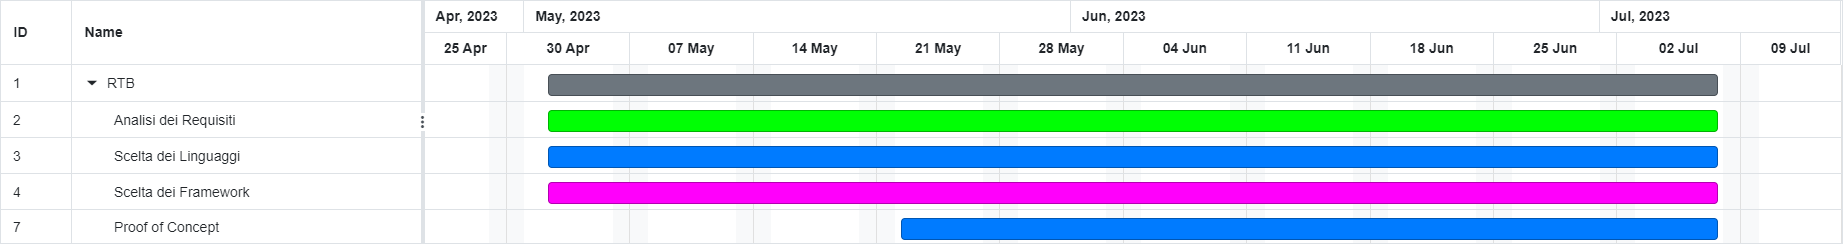
\includegraphics[scale=0.24]{RTB_1.png}\newline
\newline
\begin{tabular}{|c|c|c|c|c|c|c|c|}
    \hline
    \textbf{ORE} & \textbf{Respon.} & \textbf{Amministr.} & \textbf{Analista} & \textbf{Proget.} & \textbf{Program.} & \textbf{Verif.} & \textbf{Totale}\\
    \hline
    Erica & & & 2 & & & & 3(+2)\\
    \hline
    Francesco & & & 2 & & & & 3(+2)\\
    \hline
    Lorenzo & & & & & & 2 & 3(+2)\\
    \hline
    Matteo & & 3 & & & & & 5(+3)\\
    \hline
    Nicolas & 3 & & & & & & 4.30(+3)\\
    \hline
    Romina & & 2 & & & & & 3(+2)\\
    \hline
    \textbf{Totale} & 5(+3) & 7.30(+5) & 6(+4) & 0(+0) & 0(+0) & 3(+2) & 21.30(+14)\\
    \hline
\end{tabular}\\[8pt]

\subsubsection{Sprint 3}
\textbf{Data di inizio:} 09/05/2023\newline
\textbf{Data di fine:} 16/05/2023\newline
\newline
\textbf{Suddivisione del lavoro:}
\begin{itemize}
    \item aggiornamento dell'Analisi dei Requisiti inserendo vincoli, riferimenti normativi, riferimenti informativi e una tabella dei requisiti;
    \item aggiornamento delle Norme di Progetto inserendo una sequenza chiara per la gestione dei commit;
    \item fare uno confronto dei possibili linguaggi che si andranno poi ad utilizzare nel progetto.
\end{itemize}
\textbf{Difficoltà incontrate:}
\begin{itemize}
    \item gestione della repository;
    \item scarsa conoscenza dei comandi nel VCS;
    \item difficoltà nella scelta dei linguaggi framework data la poca esperienza accomulata e la grande presenza di alternative.
\end{itemize}
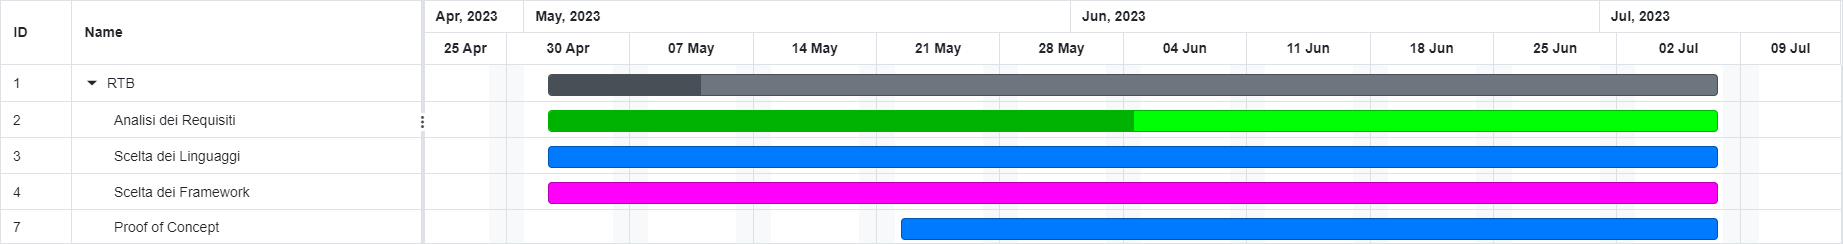
\includegraphics[scale=0.24]{RTB_2.png}\newline
\newline
\begin{tabular}{|c|c|c|c|c|c|c|c|}
    \hline
    \textbf{ORE} & \textbf{Respon.} & \textbf{Amministr.} & \textbf{Analista} & \textbf{Proget.} & \textbf{Program.} & \textbf{Verif.} & \textbf{Totale}\\
    \hline
    Erica & & 2 & & & & & 5(+2)\\
    \hline
    Francesco & & & 2 & & & & 5(+2)\\
    \hline
    Lorenzo & & 2 & & & & & 5(+2)\\
    \hline
    Matteo & 2 & & & & & & 7(+2)\\
    \hline
    Nicolas & & & & & & 2 & 6.30(+2)\\
    \hline
    Romina & & & 2 & & & & 5(+2)\\
    \hline
    \textbf{Totale} & 7(+2) & 11.30(+4) & 10(+4) & 0(+0) & 0(+0) & 5(+2) & 33.30(+12)\\
    \hline
\end{tabular}\\[8pt]

\subsubsection{Sprint 4}
\textbf{Data di inizio:} 17/05/2023\newline
\textbf{Data di fine:} 25/05/2023\newline
\newline
\textbf{Suddivisione del lavoro:}
\begin{itemize}
    \item incontro con il proponente per sistemare gli use case;
    \item inizio della stesura del \textit{Proof of Concept};
    \item decidere i linguaggi e i framework da utilizzare.
\end{itemize}
\textbf{Difficoltà incontrate:}
\begin{itemize}
    \item difficoltà nella decisione dei linguaggi da utilizzare, in quanto
    ciascun membro del gruppo ha espresso preferenze ed opinioni diverse;
    \item difficoltà nell'interpretazione di alcuni Use Case, in particolare
    nella definizione dei ruoli degli attori. 
\end{itemize}
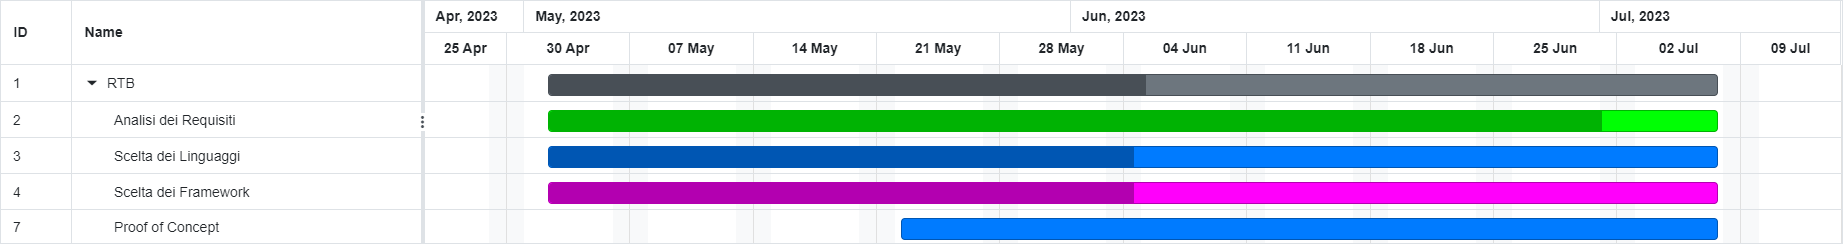
\includegraphics[scale=0.24]{RTB_3.png}\newline
\newline
\begin{tabular}{|c|c|c|c|c|c|c|c|}
    \hline
    \textbf{ORE} & \textbf{Respon.} & \textbf{Amministr.} & \textbf{Analista} & \textbf{Proget.} & \textbf{Program.} & \textbf{Verif.} & \textbf{Totale}\\
    \hline
    Erica & & 1 & & & & & 6(+1)\\
    \hline
    Francesco & & & & & & 1 & 6(+1)\\
    \hline
    Lorenzo & & 1 & & & & & 6(+1)\\
    \hline
    Matteo & & & 2 & & & & 9(+2)\\
    \hline
    Nicolas & & & 2 & & & & 8.30(+2)\\
    \hline
    Romina & 1 & & & & & & 6(+1)\\
    \hline
    \textbf{Totale} & 8(+1) & 13.30(+2) & 14(+4) & 0(+0) & 0(+0) & 6(+1) & 41.30(+8)\\
    \hline
\end{tabular}\\[8pt]

\subsubsection{Sprint 5}
\textbf{Data di inizio:} 26/05/2023\newline
\textbf{Data di fine:} 02/06/2023\newline
\newline
\textbf{Suddivisione del lavoro:}
\begin{itemize}
    \item Incontro con il professor Cardin per discutere di alcuni dubbi sugli use case;
    \item Avanzamento del \textit{Proof of Concept};
    \item Aggiornamento dell'analisi dei requisiti.
\end{itemize}
\textbf{Difficoltà incontrate:}
\begin{itemize}
    \item Alcune difficoltà nella precisa definizione di alcuni sottocasi negli use case;
    \item Difficoltà nella comprensione del funzionamento di \textit{typescript} soprattutto nel dialogo tra client e server.
\end{itemize}
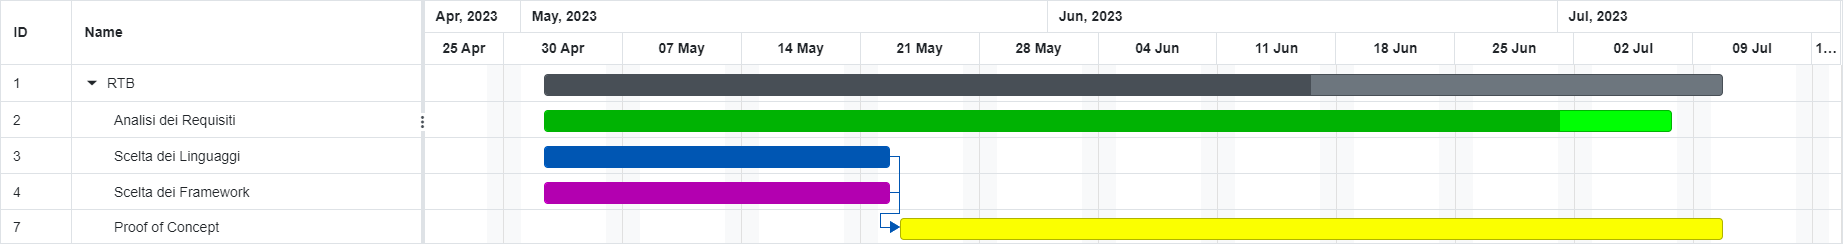
\includegraphics[scale=0.24]{RTB_4.png}\newline
\newline
\begin{tabular}{|c|c|c|c|c|c|c|c|}
    \hline
    \textbf{ORE} & \textbf{Respon.} & \textbf{Amministr.} & \textbf{Analista} & \textbf{Proget.} & \textbf{Program.} & \textbf{Verif.} & \textbf{Totale}\\
    \hline
    Erica & 1 & & 2 & & & & 9(+3)\\
    \hline
    Francesco & & & & & & 1 & 7(+1)\\
    \hline
    Lorenzo & & & & & & 1 & 7(+1)\\
    \hline
    Matteo & & & & & 2 & & 11(+2)\\
    \hline
    Nicolas & & & & & 2 & & 10.30(+2)\\
    \hline
    Romina & & & 2 & & & & 8(+2)\\
    \hline
    \textbf{Totale} & 9(+1) & 13.30(+0) & 18(+4) & 0(+0) & 4(+4) & 8(+2) & 52.30(+11)\\
    \hline
\end{tabular}\\[8pt]

\subsubsection{Sprint 6}
\textbf{Data di inizio:} 03/06/2023\newline
\textbf{Data di fine:} 12/06/2023\newline
\newline
\textbf{Suddivisione del lavoro:}
\begin{itemize}
    \item Completare il \textit{Glossario} con eventuali termini mancanti;
    \item Chiedere al proponente un controllo dell'\textit{Analisi dei Requisiti};
    \item Avanzamento del \textit{Proof of Concept}.
\end{itemize}
\textbf{Difficoltà incontrate:}
\begin{itemize}
    \item Eseguire il \textit{Proof of Concept} nella macchina locale di ogni componente del gruppo, dovuto alla mancanza di alcuni pacchetti fondamentali per l'esecuzione del codice.
\end{itemize}
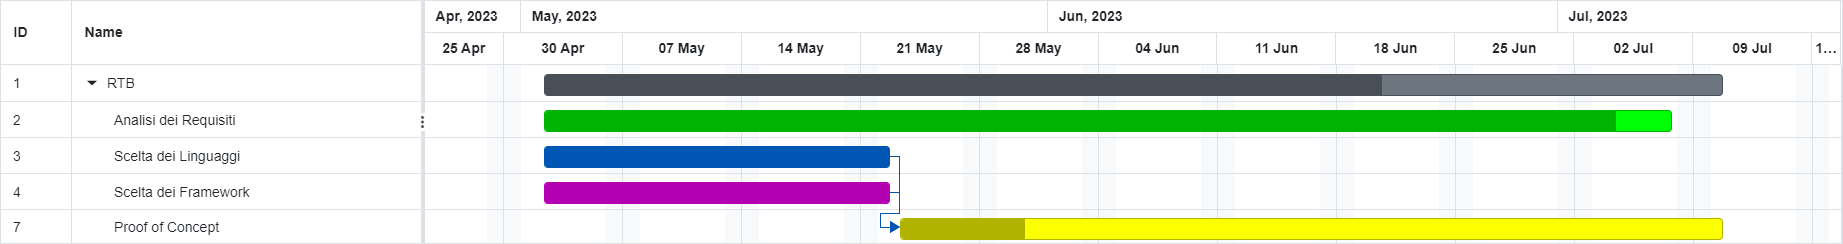
\includegraphics[scale=0.24]{RTB_5.png}\newline
\newline
\begin{tabular}{|c|c|c|c|c|c|c|c|}
    \hline
    \textbf{ORE} & \textbf{Respon.} & \textbf{Amministr.} & \textbf{Analista} & \textbf{Proget.} & \textbf{Program.} & \textbf{Verif.} & \textbf{Totale}\\
    \hline
    Erica & & & & & & 2 & 11(+2)\\
    \hline
    Francesco & & & 2 & & & & 9(+2)\\
    \hline
    Lorenzo & & & 2 & & & & 9(+2)\\
    \hline
    Matteo & & & & & 3 & & 14(+3)\\
    \hline
    Nicolas & & 0.30 & & & 2 & & 13(+2.30)\\
    \hline
    Romina & 2 & & & & & & 10(+2)\\
    \hline
    \textbf{Totale} & 11(+2) & 14(+0.30) & 22(+4) & 0(+0) & 10(+6) & 11(+2) & 66(+13.30)\\
    \hline
\end{tabular}\\[8pt]

\subsubsection{Sprint 7}
\textbf{Data di inizio:} 13/06/2023\newline
\textbf{Data di fine:} 19/06/2023\newline
\newline
\textbf{Suddivisione del lavoro:}
\begin{itemize}
    \item Avanzamento dello sviluppo del \textit{Proof of Concept}.
\end{itemize}
\textbf{Difficoltà incontrate:}
\begin{itemize}
    \item Eseguire correttamente il codice all'interno di un \textit{container Docker};
    \item Integrazione del database \textit{MongoDB} con il codice presente.
\end{itemize}
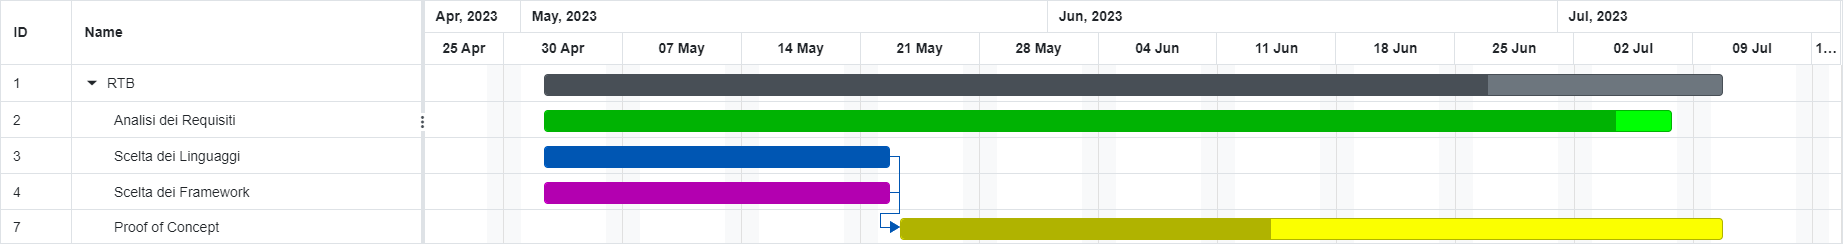
\includegraphics[scale=0.24]{RTB_6.png}\newline
\newline
\begin{tabular}{|c|c|c|c|c|c|c|c|}
    \hline
    \textbf{ORE} & \textbf{Respon.} & \textbf{Amministr.} & \textbf{Analista} & \textbf{Proget.} & \textbf{Program.} & \textbf{Verif.} & \textbf{Totale}\\
    \hline
    Erica & & & & & 2 & & 13(+2)\\
    \hline
    Francesco & & & & 2 & & & 11(+2)\\
    \hline
    Lorenzo & 1 & & & & & & 10(+1)\\
    \hline
    Matteo & & & & 1 & & & 15(+1)\\
    \hline
    Nicolas & & & 2 & & & & 15(+2)\\
    \hline
    Romina & & 1 & & & & & 11(+1)\\
    \hline
    \textbf{Totale} & 12(+1) & 15(+1) & 24(+2) & 3(+3) & 12(+2) & 11(+0) & 75(+9)\\
    \hline
\end{tabular}\\[8pt]

\subsubsection{Sprint 8}
\textbf{Data di inizio:} 19/06/2023\newline
\textbf{Data di fine:} 03/07/2023\newline
\newline
\textbf{Suddivisione del lavoro:}
\begin{itemize}
    \item Avanzamento dello sviluppo del \textit{Proof of Concept}
    \begin{itemize}
        \item Implementazione del MongoDB e primo collegamento al server;
        \item Implementazione modello sensore;
        \item Implementazione modello area illuminata
    \end{itemize}
\end{itemize}
\textbf{Difficoltà incontrate:}
\begin{itemize}
    \item Eseguire correttamente il codice all'interno di un \textit{container Docker};
    \item Integrazione del database \textit{MongoDB} con il codice presente.
\end{itemize}
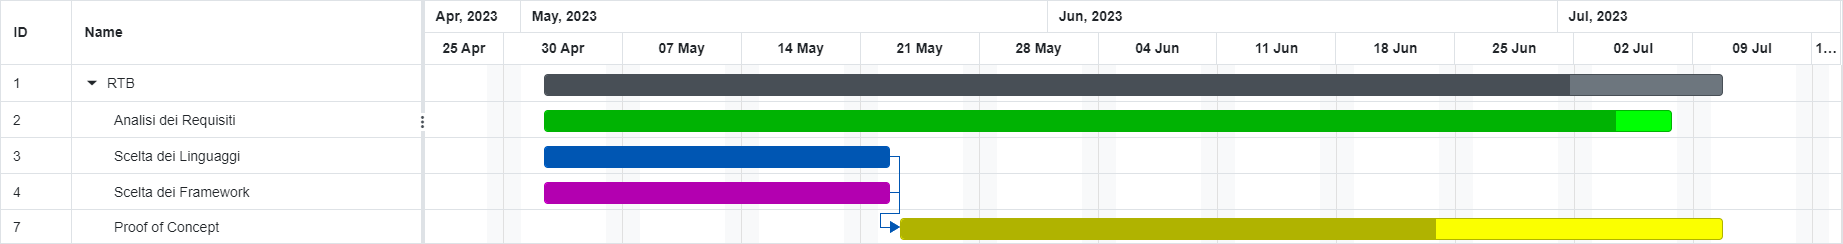
\includegraphics[scale=0.24]{RTB_7.png}\newline
\newline
\begin{tabular}{|c|c|c|c|c|c|c|c|}
    \hline
    \textbf{ORE} & \textbf{Respon.} & \textbf{Amministr.} & \textbf{Analista} & \textbf{Proget.} & \textbf{Program.} & \textbf{Verif.} & \textbf{Totale}\\
    \hline
    Erica & & & & 0.5 & & & 13.5(+0.5)\\
    \hline
    Francesco & & & & 0.5 & & & 11.5(+0.5)\\
    \hline
    Lorenzo & 1 & & & & & & 11(+1)\\
    \hline
    Matteo & & & & & & 1 & 16(+1)\\
    \hline
    Nicolas & & & & & 2 & & 17(+2)\\
    \hline
    Romina & & 1 & & & & & 12(+1)\\
    \hline
    \textbf{Totale} & 13(+1) & 16(+1) & 24(+0) & 4(+1) & 14(+2) & 12(+1) & 81(+6)\\
    \hline
\end{tabular}\\[8pt]

\newpage

\section{Preventivo delle ore e dei costi}

\subsection{Suddivisione delle ore previste}

\begin{tabular}{|c|c|c|c|c|c|c|c|}
    \hline
    \textbf{} & \textbf{Respon.} & \textbf{Amministr.} & \textbf{Analista} & \textbf{Proget.} & \textbf{Program.} & \textbf{Verif.} & \textbf{Totale}\\
    \hline
    Erica & 11 & 9 & 17 & 21 & 22 & 15 & 95\\
    \hline
    Francesco & 12 & 8 & 16 & 22 & 22 & 15 & 95\\
    \hline
    Lorenzo & 12 & 8 & 16 & 22 & 22 & 15 & 95\\
    \hline
    Matteo & 12 & 8 & 17 & 22 & 21 & 15 & 95\\
    \hline
    Nicolas & 11 & 9 & 17 & 22 & 21 & 15 & 95\\
    \hline
    Romina & 12 & 8 & 17 & 21 & 22 & 15 & 95\\
    \hline
    \textbf{Totale} & 70 & 50 & 100 & 130 & 130 & 90 & 570\\
    \hline
\end{tabular}\\[8pt]

\subsection{Costi attesi}

\begin{tabular}{|c|c|c|c|}
    \hline
    \textbf{Ruolo} & \textbf{Costo orario (\euro)} & \textbf{Ore} & \textbf{Prezzo (\euro)}\\
    \hline
    Responsabile & 30 & 70 & 2100\\
    \hline
    Amministratore & 20 & 50 & 1000\\
    \hline
    Analista & 25 & 100 & 2500\\
    \hline
    Progettista & 25 & 130 & 3250\\
    \hline
    Programmatore & 15 & 130 & 1950\\
    \hline
    Verificatore & 15 & 90 & 1350\\
    \hline\hline
    \multicolumn{2}{|c|}{\textbf{Scadenza consegna}} & \textbf{Ore tot.} & \textbf{Preventivo finale (\euro)}\\
    \hline
    \multicolumn{2}{|c|}{15/09/2023} & 570 & 12150\\
    \hline
\end{tabular}\\[8pt]

\subsection{Grafico dei costi attesi}
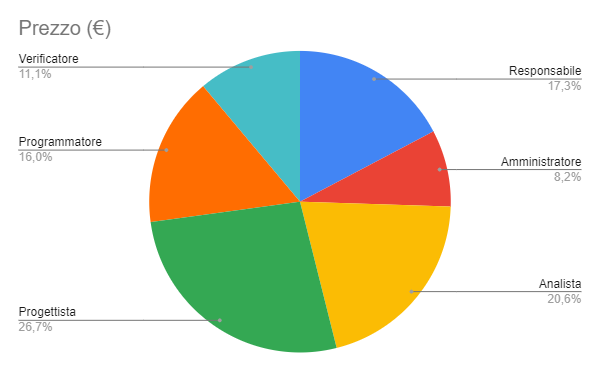
\includegraphics{grafico_costi.png}

\end{document}
